%----------------------------------------------------------------------------------------------------
\section{Results}

%--------------------------------------------------
% the results drawn from the optimised binning

\begin{figure}
\begin{center}
% Do not scale the graphics - fonts have been adjusted to match with figure caption.
% If needed, ask for a different size at jan.kaspar@cern.ch.
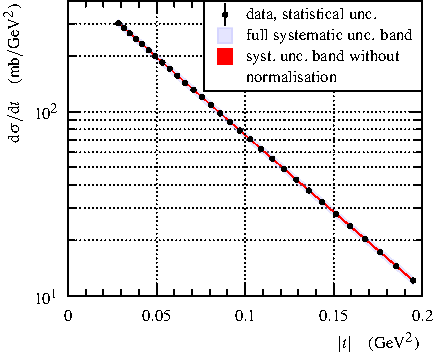
\includegraphics{fig/t_dist.pdf}
\caption{%
Differential cross-section using ``optimised'' binning, as given in Table~\ref{tab:data}.
}
\label{fig:data ob}
\end{center}
\end{figure}


The final differential cross-section in the ``optimised'' binning is presented in Table~\ref{tab:data} and Figure \ref{fig:data ob}. In order to visualise small deviations from the leading pure-exponential behaviour, Figure~\ref{fig:data rel ob} shows the relative difference of the cross-section from a reference exponential. This plot immediately suggests a non-exponentiality of the data: pure exponentials would look like (almost) linear functions in this reference frame.

To study the detailed behaviour of the differential cross-section, a series of fits has been made using the parametrisation:
\begin{equation}
\label{eq:fit param}
{\d\sigma\over\d t}(t) = \left. \d\sigma\over\d t\right|_{0} \ \exp\left( \sum\limits_{i = 1}^{N_{b}} b_i\, t^i \right) \ ,
\end{equation}
which includes the pure exponential ($N_b = 1$) and its straight-forward extensions ($N_b = 2, 3$).

The fits have been performed by the standard least-squares method, in particular minimising:
\begin{equation}
\label{eq:chi sq}
\chi^2 = \Delta^\T \mat V^{-1} \Delta\ ,\quad \Delta = (\hbox{data} - \hbox{fit})\ ,\quad \mat V = \mat V_{\rm stat} + \mat V_{\rm syst}\ ,
\end{equation}
where $\Delta$ is a vector of differences between the differential cross-section data and a fit function evaluated at the bin representative points (see Table~\ref{tab:data}). The covariance matrix $\mat V$ is given by the sum of the statistical component $\mat V_{\rm stat}$ (statistical uncertainty from Table~\ref{tab:data} on the diagonal) and the systematic component $\mat V_{\rm stat}$ (see Eq.~(\ref{eq:covar mat})).

The quality of fits is judged on the basis of several measures. The first is the value of $\chi^2$ after minimisation divided by the number of degrees of freedom (ndf). Secondly, the p-value stands for the probability that a $\chi^2$ value greater than the observed one would be drawn from the $\chi^2$ distribution with the given number of degrees of freedom. Eventually, significance means the half-width of a central region that needs to be excluded from a normal distribution to get the same integrated probability as the p-value. The significance is expressed in multiples of sigma, the standard deviation of the normal distribution.

Figure~\ref{fig:data rel ob} shows several fits of the differential cross-section with the parametrisation in Eq.~(\ref{eq:fit param}) and different numbers of parameters in the exponent, $N_b$. The corresponding fit quality is given in Table~\ref{tab:fits ob}, indicating that the purely exponential fit ($N_b = 1$) is excluded at $7.2\un{\sigma}$ significance.
%
The other two fits ($N_b = 2, 3$) are of reasonable quality and can, therefore, be used for a total cross-section estimation with the optical theorem in the form
\begin{equation}
\label{eq:si tot}
\sigma_{\rm tot}^2 = {16\pi\, (\hbar c)^2\over 1 + \rho^2}\, \left. \d\sigma_{\rm el}\over\d t\right|_0\ ,
\end{equation}
for the first time using a non-exponential extrapolation to $t=0$. Using the COMPETE~\cite{compete} preferred-model extrapolation of $\rho = 0.140\pm 0.007$ yields
\begin{equation}
\label{eq:si tot results}
	\begin{aligned}
		N_b &= 2:\quad \sigma_{\rm tot} = (100.8 \pm 2.1)\un{mb}\ ,\\	% A = 529.3 +- 21.9
		N_b &= 3:\quad \sigma_{\rm tot} = (101.2 \pm 2.1)\un{mb}\ ,\\	% A = 533.5 +- 21.9
	\end{aligned}
\end{equation}
which are well compatible with the previous measurement using the luminosity-independent method~\cite{prl111}.

\begin{table}
\caption{%
Fit quality measures for fits in Figure~\ref{fig:data rel ob}.
}
\vskip-2mm
\label{tab:fits ob}
\begin{center}
\small
\begin{tabular}{cccc}
\hline
\hline
$N_b$ & $\chi^2/\hbox{ndf}$ & p-value & significance\cr
\hline
$1$ & $117.5/28 = 4.20$ & $6.1\cdot 10^{-13}$ & $7.2\un{\sigma}$ \cr
$2$ & $29.3/27 = 1.09$ & $0.35$ & $0.94\un{\sigma}$ \cr
$3$ & $25.5/26 = 0.98$ & $0.49$ & $0.69\un{\sigma}$ \cr
\hline
\hline
\end{tabular}
\end{center}
\end{table}


\begin{figure*}
\vskip-5mm
\begin{center}
% Do not scale the graphics - fonts have been adjusted to match with figure caption.
% If needed, ask for a different size at jan.kaspar@cern.ch.
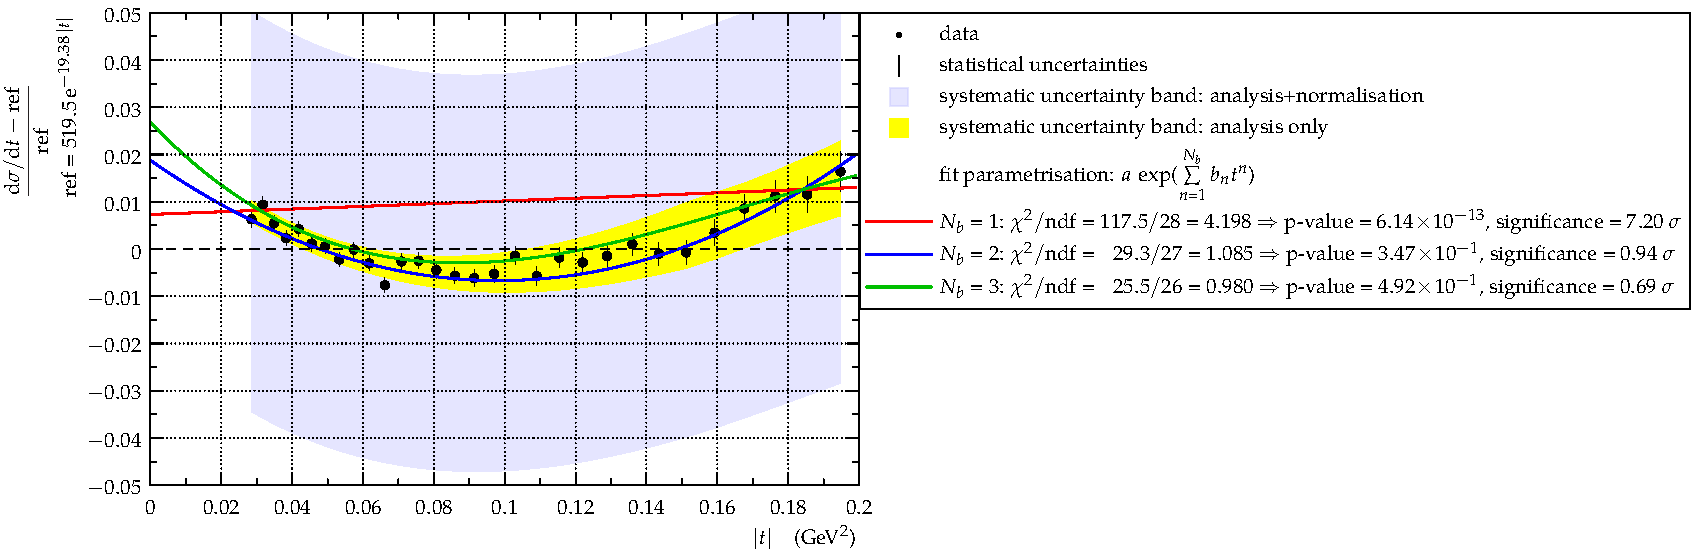
\includegraphics{fig/t_dist_rel_with_fits.pdf}
\vskip-4mm
\caption{%
Differential cross-section using the ``optimised'' binning and plotted as relative difference from a reference exponential (see vertical axis). The black dots represent data points with statistical uncertainty bars. The coloured lines correspond to fits with parametrisation Eq.~(\ref{eq:fit param}) and different numbers of parameters in the exponent. The red line lies seemingly too high with respect to the data points, which is a consequence of the systematic degrees of freedom included in the fit. The blue band corresponds to the full systematic uncertainty, the yellow one includes all systematic contributions except the normalisation. Both bands are centred around the fit curve with $N_b = 3$.
}
\label{fig:data rel ob}
\end{center}
\vskip-2mm
\end{figure*}


%--------------------------------------------------
% results from per-mille binning

The incompatibility between a pure-exponential behaviour and the data with the ``per-mille'' binning can be shown equally well. However, since the number of points is drastically increased, the straight-forward $\chi^2$ test does not have sufficient sensitivity, and a different test is used. Assuming that the data can be described by a pure exponential, the fit parameters should have compatible values for fits over different ranges. Figure~\ref{fig:data rel cpb0.001} shows a fit (minimisation of $\chi^2$ from Eq.~(\ref{eq:chi sq})) with the parametrisation
\begin{equation}
\label{eq:split fit param}
{\d\sigma\over\d t}(t) =
\begin{cases}
a_1\, \e^{b_1 |t|} & |t| < 0.07\un{GeV^2}\\
a_2\, \e^{b_2 |t|} & |t| > 0.07\un{GeV^2}\\
\end{cases}
\end{equation}
giving a reasonable fit quality (p-value of 0.57). The compatibility of the parameters in the two $|t|$ regions can be verified by evaluating
\begin{equation}
\label{eq:chi sq param}
\chi_p^2 = \Delta_p^\T \mat V_p^{-1} \Delta_p\ ,\quad \Delta_p =
\begin{pmatrix}
a_1 - a_2\\
b_1 - b_2\\
\end{pmatrix}\ ,
\end{equation}
where $\mat V_p$ is the covariance matrix for the difference vector $\Delta_p$. It yields $\chi_p^2 = 65.4$ which with $2$ degrees of freedom corresponds to a p-value of $6.2\cdot10^{-15}$ and a significance of $7.8\un{\sigma}$. This, in turn, rules out the hypothesis of a purely exponential behaviour of the data over the entire observed range.


\iffalse
 A1 − A2 = 14.617 ± 1.789 ⇒ 8.2 σ
 B1 − B2 = −0.414 ± 0.056 ⇒ 7.4 σ
\fi

Since parameters estimated with the least squares method are unbiased, the test in Eq.~(\ref{eq:chi sq param}) is asymptotically binning independent. Indeed, applying it to the data in the ``optimised'' binning (prior to the statistical uncertainty rescaling, Section \ref{sec:stat unc adj}) yields $\chi^2_p = 65.7$ which corresponds to a significance of $7.8\un{\sigma}$. After the uncertainty rescaling, the exclusion significance increases to $9.0\un{\sigma}$.

\iffalse
DS4-sc, ob

A1 - A2 = 14.273 +- 1.549
B1 - B2 = -0.421 +- 0.051

S2 = 8.519790E+01
prob_A+B = 3.158714E-19

>> significances
        A: 9.2
        B: -8.2
        A+B: 9.0
\fi

\iffalse
DS4, ob

A1 - A2 = 14.501 +- 1.789
B1 - B2 = -0.426 +- 0.059

S2 = 6.574304E+01
prob_A+B = 5.297602E-15

>> significances
        A: 8.1
        B: -7.2
        A+B: 7.8
\fi

\begin{figure*}
\begin{center}
% Do not scale the graphics - fonts have been adjusted to match with figure caption.
% If needed, ask for a different size at jan.kaspar@cern.ch.
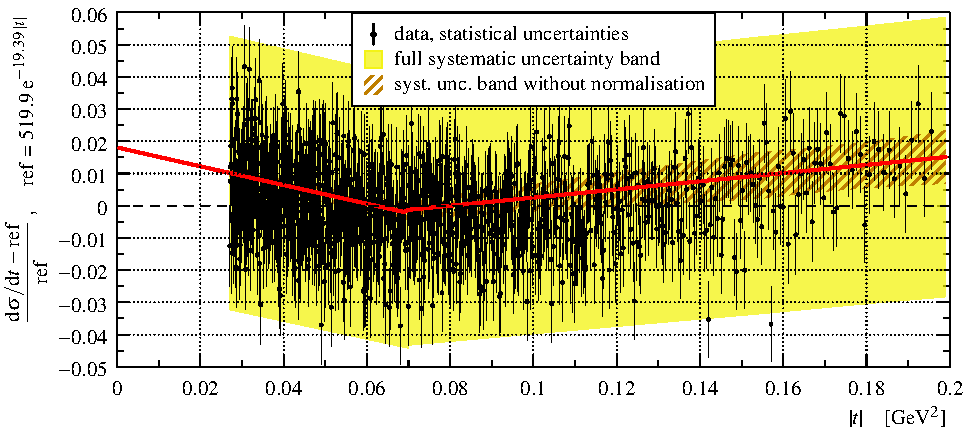
\includegraphics{fig/t_dist_rel_with_split_fit.pdf}
\vskip-4mm
\caption{%
Differential cross-section using the ``per-mille'' binning and plotted as relative difference from the reference exponential (see vertical axis). The black dots represent data points with statistical uncertainty bars. The red line shows pure exponential fits in regions below and above $|t| = 0.07\un{GeV^2}$, see Eq.~(\ref{eq:split fit param}). The blue band corresponds to the full systematic uncertainty, the yellow one includes all systematic contributions except the normalisation. Both bands are centred around the fit curve.
}
\label{fig:data rel cpb0.001}
\end{center}
\end{figure*}

